\documentclass[11pt, a4paper, reqno]{scrartcl}

\usepackage[utf8]{inputenc}
\usepackage{a4wide}
\usepackage{libertine}
\usepackage{graphicx}
\usepackage{listings}
\usepackage{xcolor}
\usepackage{float}
\usepackage{amsmath}
\usepackage{microtype}
\usepackage{hyperref}
\usepackage{pdflscape}

% for latex output of pandas
\usepackage{booktabs}

\begin{document}
    \title{Exercise No. 9}
    \author{David Bubeck, Pascal Becht, Patrick Nisbl\`e}
    \maketitle

    \lstset{
        language=Python,
        backgroundcolor=\color{gray!5},
        numbers=left,
        captionpos=t,
        breaklines=true,
        frame=l,
        xleftmargin=\parindent,
        basicstyle=\footnotesize\sffamily,
        keywordstyle=\bfseries\color{green!40!black},
        commentstyle=\itshape\color{purple!40!black},
        identifierstyle=\color{blue!60!black},
        stringstyle=\color{orange}
    }

    \section{2 - The Lorenz attractor}
   
    	The Lorenz attractor problem is given by the following coupled set of 				differentail equations:
    	\begin{align}
    		\dot{x} = -\sigma (x - y) \\
    		\dot{y} = rx - y - xz \\
    		\dot{z} = xy - bz
    	\end{align}
    	Our fixed points are $(0, 0, 0)$ for all $r$ and $C_{\pm} = (\pm a_0, \pm 			a_0, r - 1)$ with $a_0 = \sqrt{b(r - 1}$ for $r > 1$. For this exercise we 			use $\sigma = 10$ and $b = \frac{8}{3}$.
    
     \subsection*{a)}
     	Using rk4 we solve the set of equations above numerically for $r = 0.5, 			1.15, 1.3456, 24$ and $30$.
     	
     	Following is the code for rk4 calculation:
     	\begin{figure}[H]
     		\lstinputlisting[lastline=46]{rk4.py}
     	\end{figure}
     	
     	The problem will be solved with:
     	\begin{figure}[H]
     		\lstinputlisting[lastline=44]{09-1.py}
     	\end{figure}
    
    	Here are the plots for the solutions given with the code above
        \begin{figure}
        	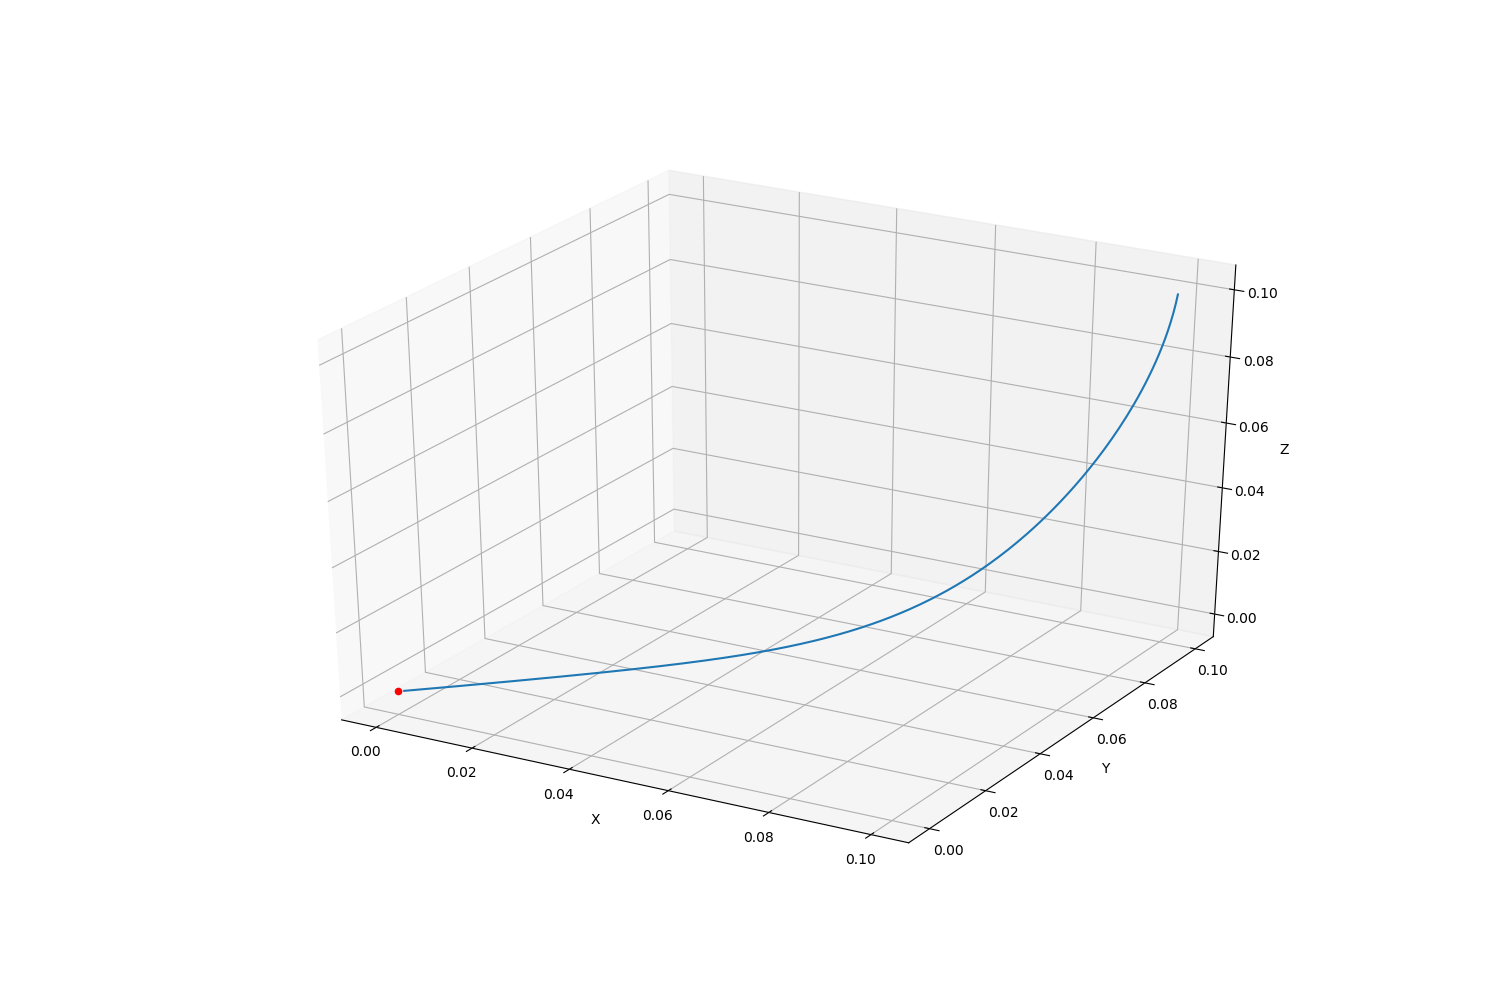
\includegraphics[scale = 0.25]{plot_0.png}
            \caption{r = 0.5}
            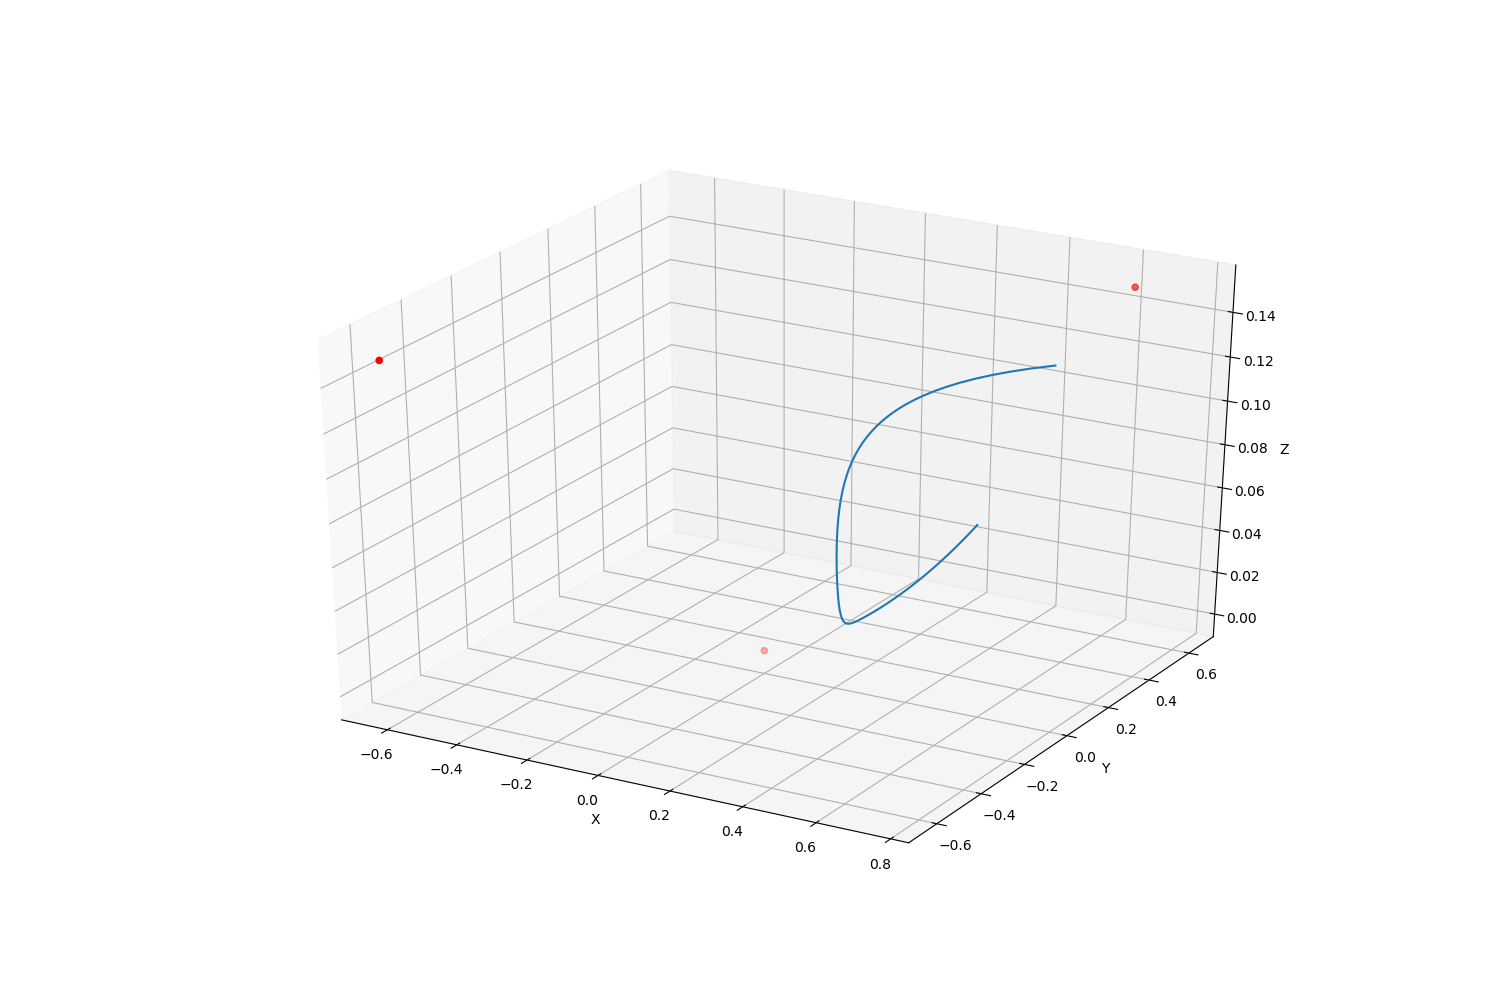
\includegraphics[scale = 0.25]{plot_1.png}
            \caption{r = 1.15}
            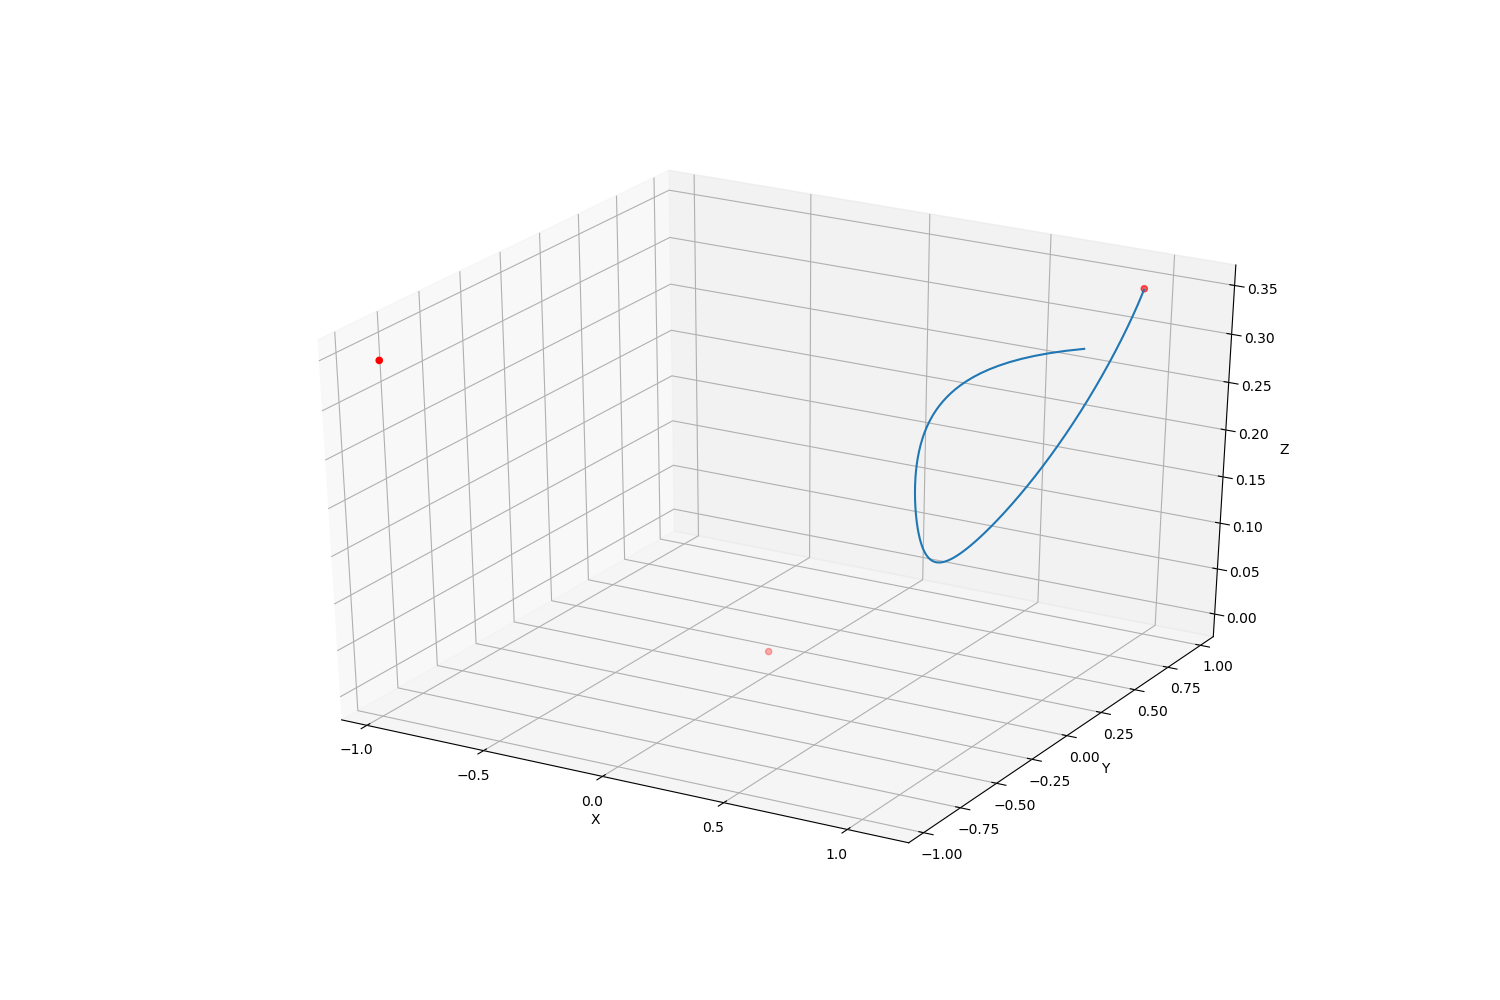
\includegraphics[scale = 0.25]{plot_2.png}
            \caption{r = 1.3456}
        \end{figure}
        \begin{figure}
        	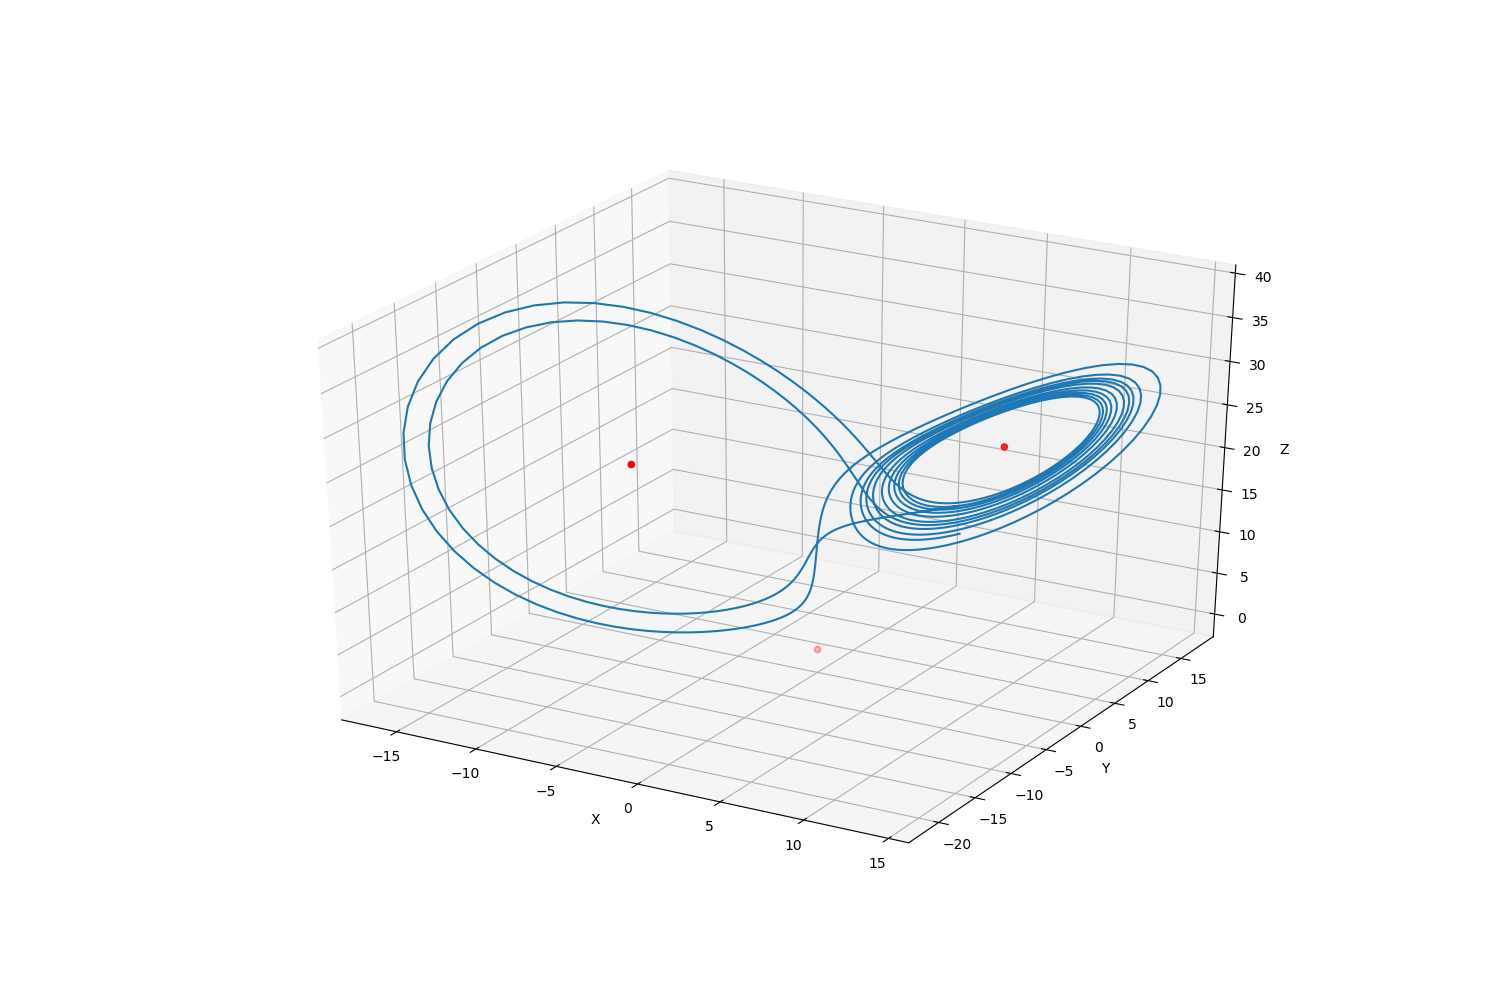
\includegraphics[scale = 0.25]{plot_3.png}
            \caption{r = 24}
            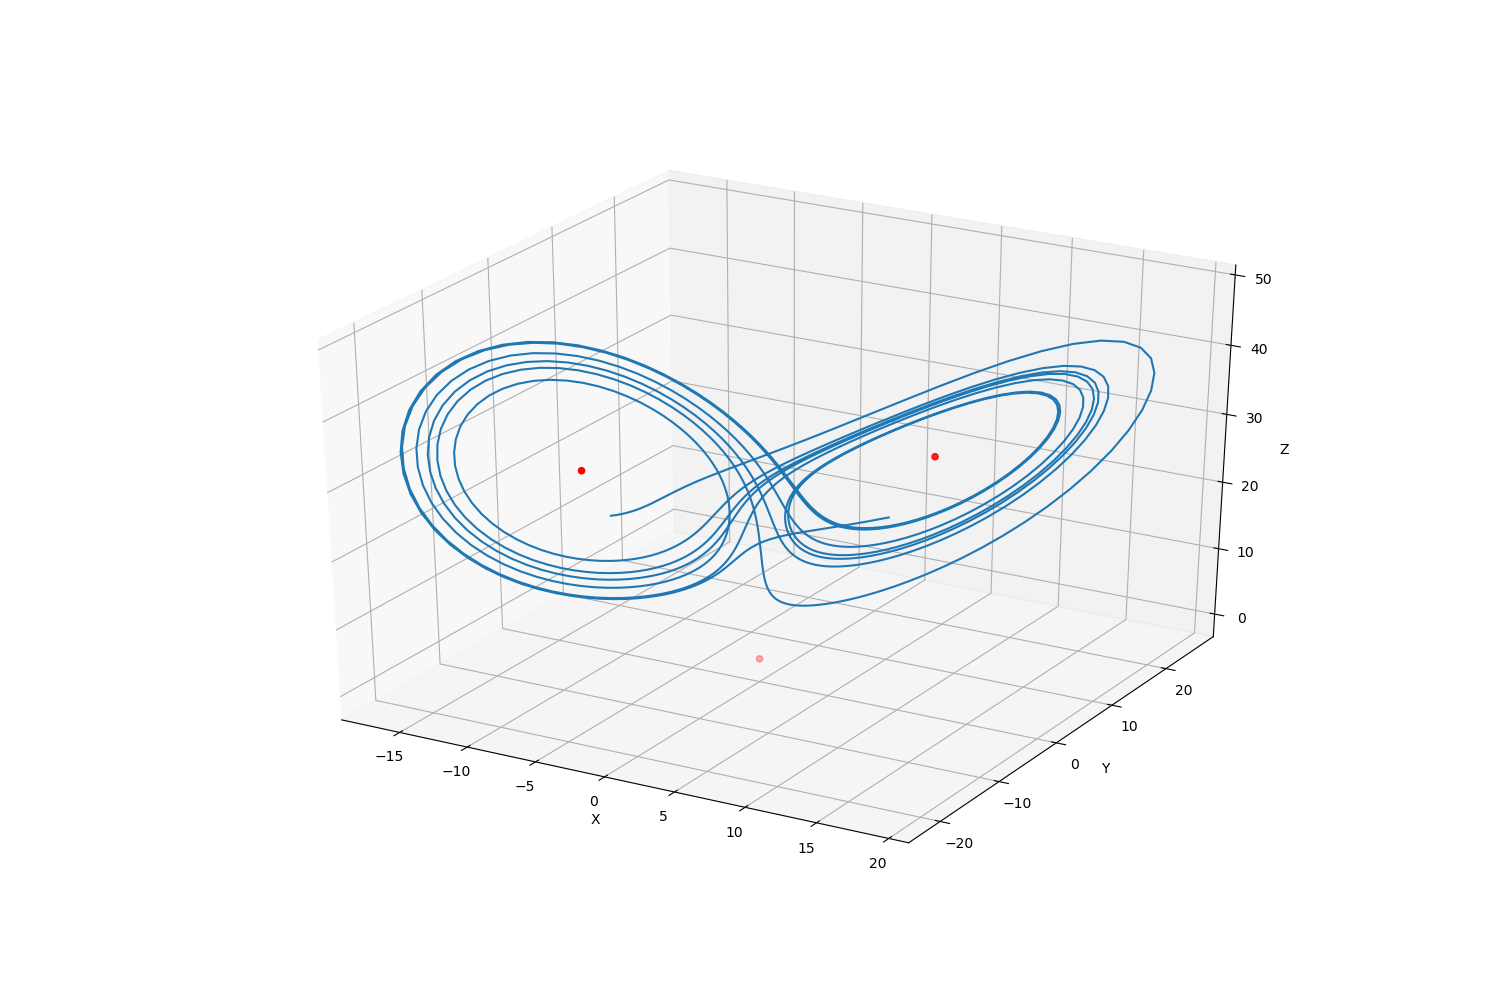
\includegraphics[scale = 0.25]{plot_4.png}
            \caption{r = 26}
            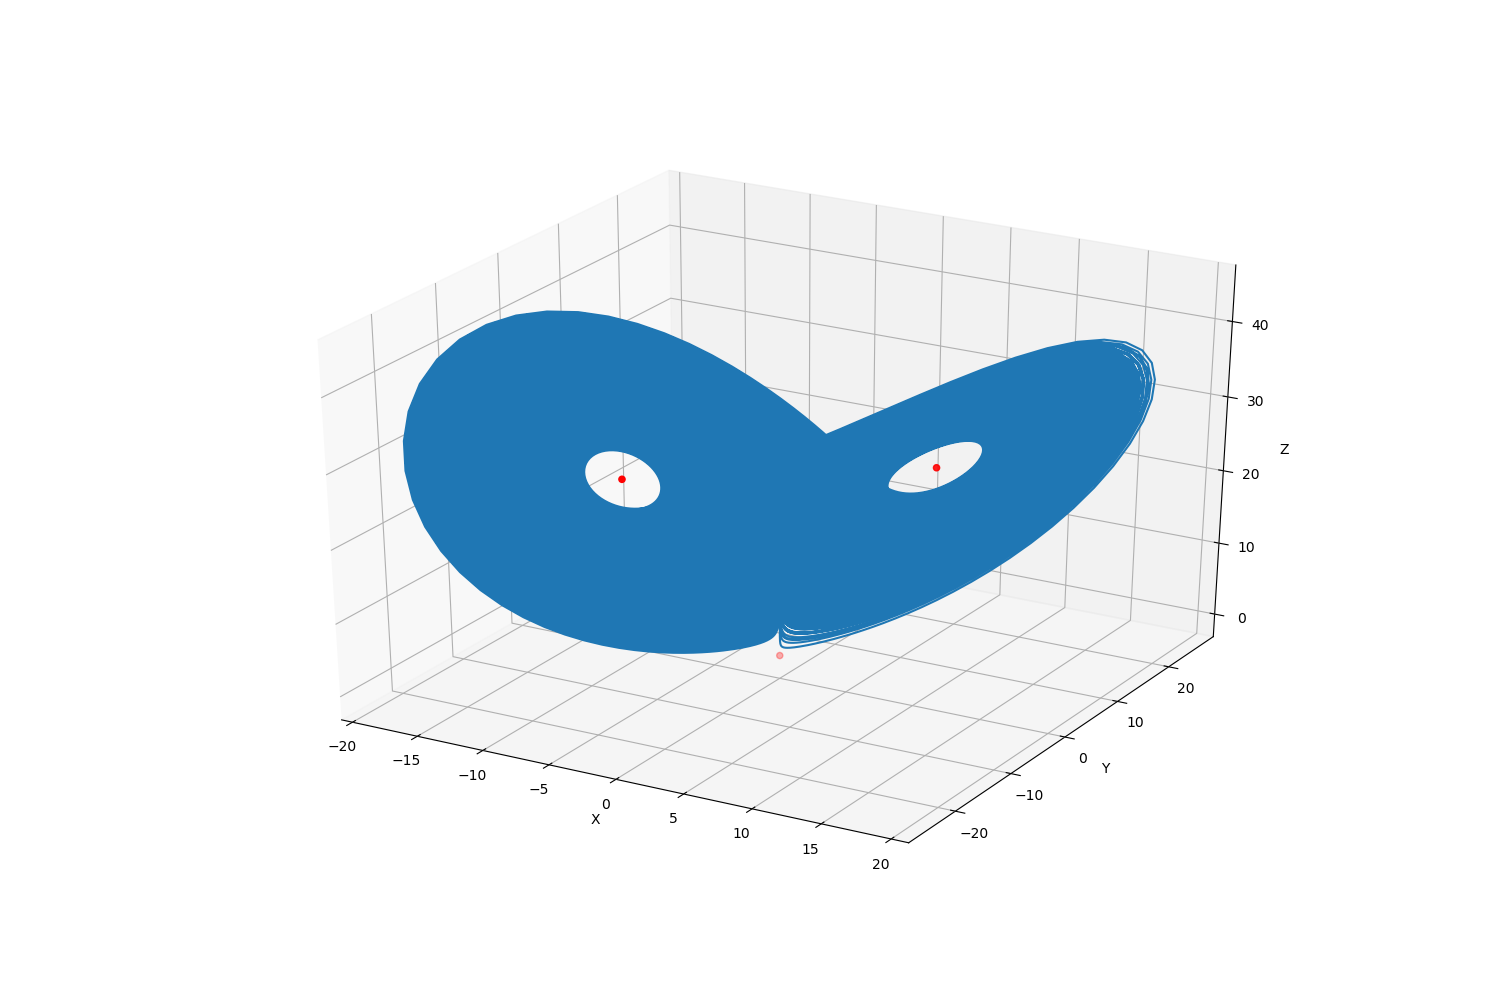
\includegraphics[scale = 0.25]{plot_5.png}
            \caption{r = 30}
        \end{figure}
        
        In figure 1 you can see that the function converge fast against point $(0, 			0, 0)$ in which lies our fix point. In figure 2 our function converge also 			against a fix point, but here it is the $C_+$ fix point. All following 				values lies on this point, so it is stabel. Starting at figure 4 the 				function forms \" butterfly \". The function circulates around the fix 				points but never converge. So for large r we don't have stable fix points.
        
	\subsection*{b)}
		For the second part we determine for $r = 26$ the local maximum in $z$ and 			plot $z_{k + 1}$ as a function of $z_k$
		\begin{figure}[H]
     		\lstinputlisting[lastline=51]{Exercise09_2_test.py}
     	\end{figure}
		\begin{figure}[H]
     		\lstinputlisting[firstline=52, firstnumber=52, lastline=87]{Exercise09_2_test.py}
     	\end{figure}
     	\begin{figure}
     		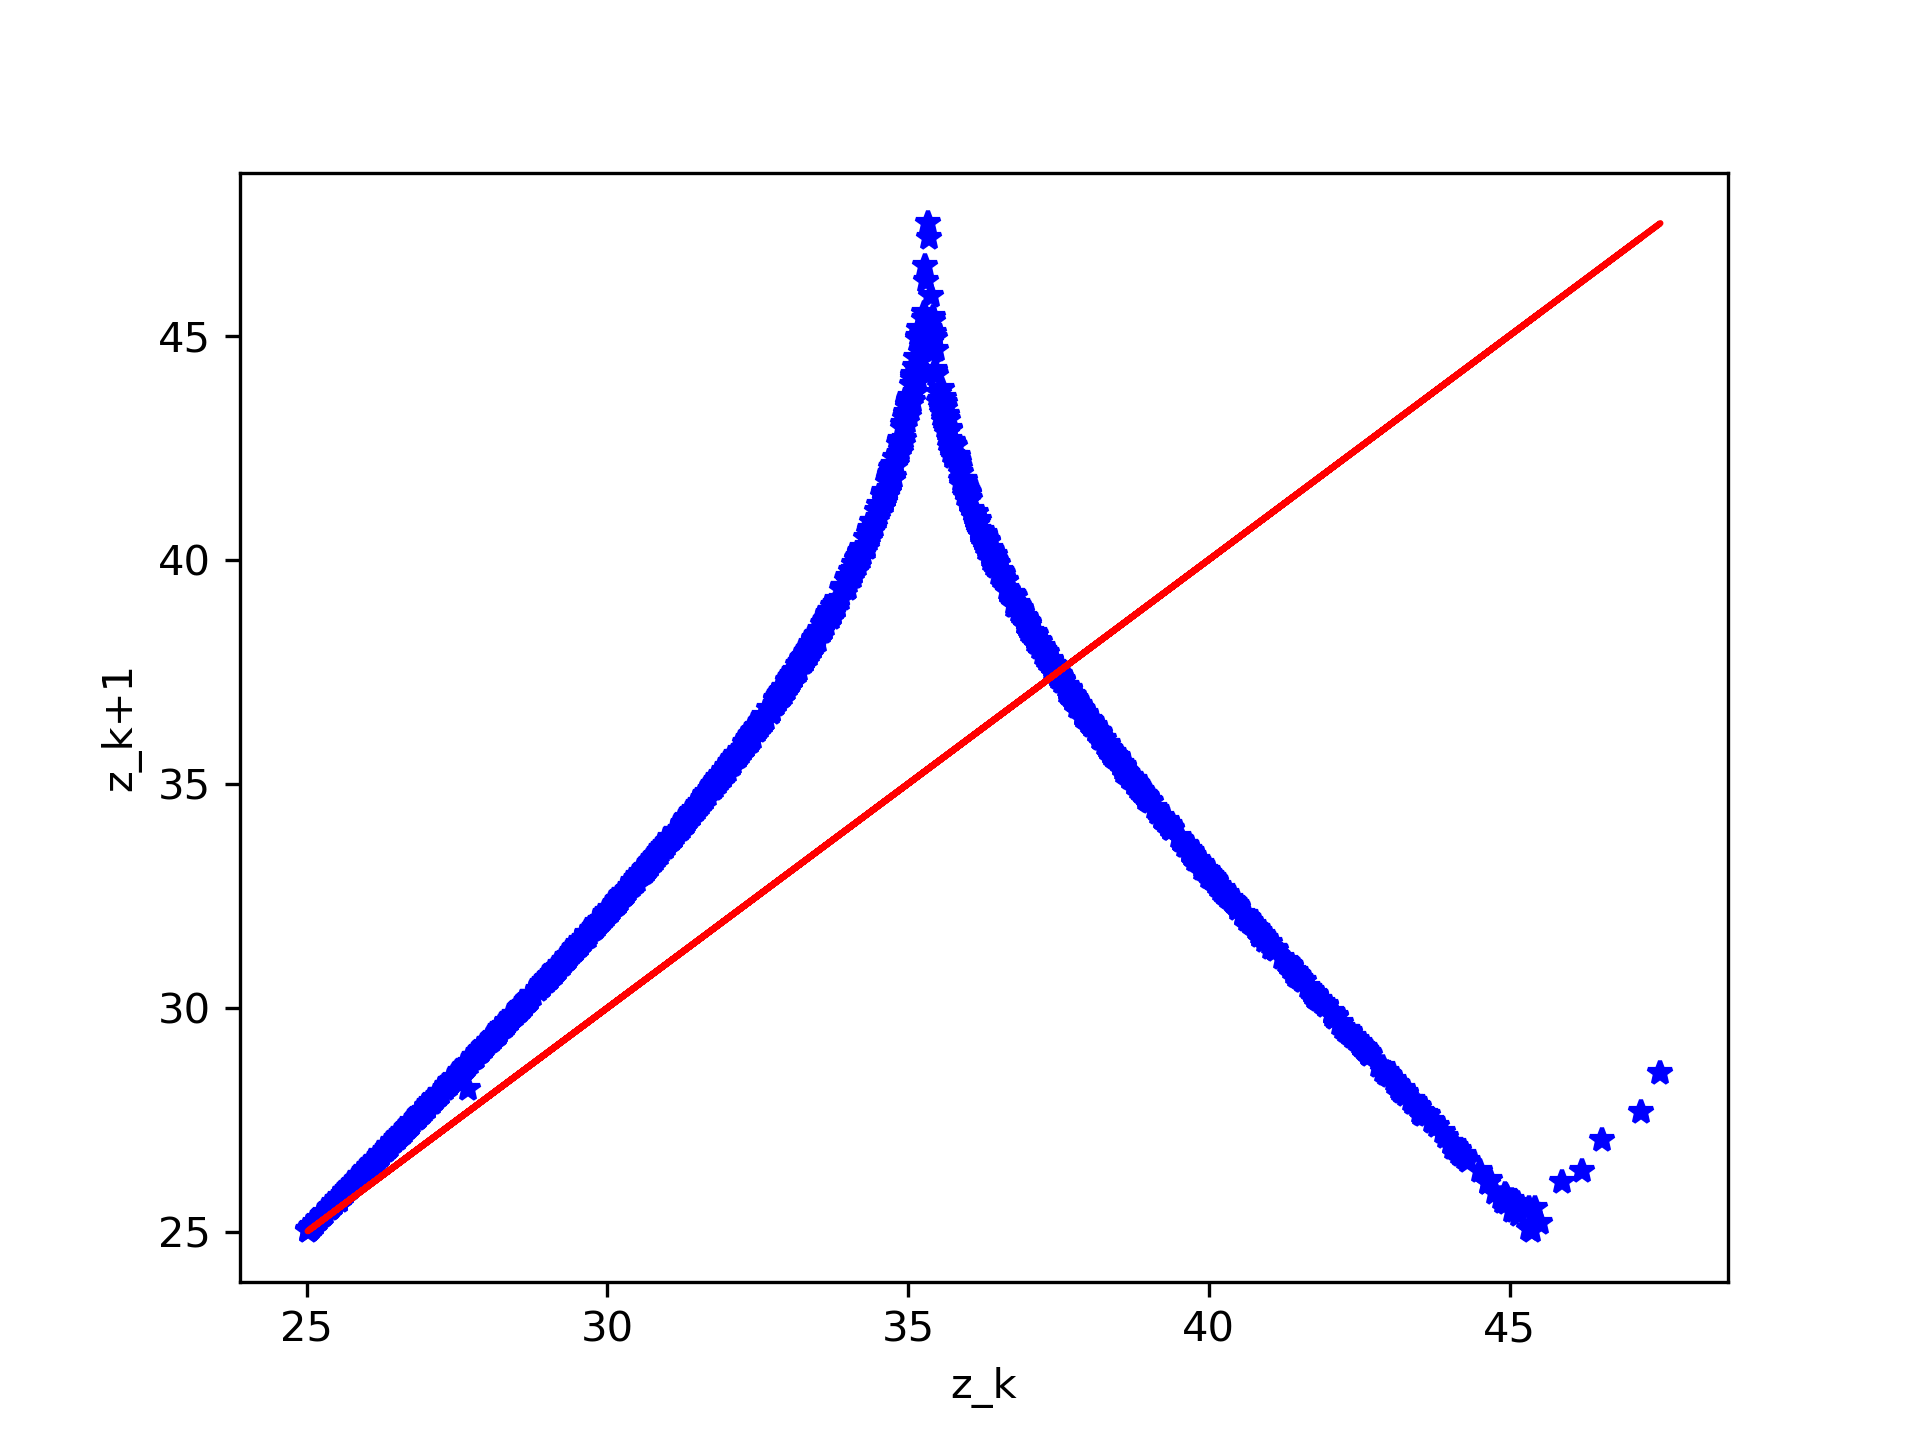
\includegraphics[scale = 1]{z_k.png}
     		\caption{r = 26}
     	\end{figure}
     	
     	We can see that the slope at the fixed point is approximately -1, which is the limit for a pereodic solution. 
      
        
        
\end{document}